% Options for packages loaded elsewhere
\PassOptionsToPackage{unicode}{hyperref}
\PassOptionsToPackage{hyphens}{url}
%
\documentclass[
]{article}
\usepackage{lmodern}
\usepackage{amssymb,amsmath}
\usepackage{ifxetex,ifluatex}
\ifnum 0\ifxetex 1\fi\ifluatex 1\fi=0 % if pdftex
  \usepackage[T1]{fontenc}
  \usepackage[utf8]{inputenc}
  \usepackage{textcomp} % provide euro and other symbols
\else % if luatex or xetex
  \usepackage{unicode-math}
  \defaultfontfeatures{Scale=MatchLowercase}
  \defaultfontfeatures[\rmfamily]{Ligatures=TeX,Scale=1}
\fi
% Use upquote if available, for straight quotes in verbatim environments
\IfFileExists{upquote.sty}{\usepackage{upquote}}{}
\IfFileExists{microtype.sty}{% use microtype if available
  \usepackage[]{microtype}
  \UseMicrotypeSet[protrusion]{basicmath} % disable protrusion for tt fonts
}{}
\makeatletter
\@ifundefined{KOMAClassName}{% if non-KOMA class
  \IfFileExists{parskip.sty}{%
    \usepackage{parskip}
  }{% else
    \setlength{\parindent}{0pt}
    \setlength{\parskip}{6pt plus 2pt minus 1pt}}
}{% if KOMA class
  \KOMAoptions{parskip=half}}
\makeatother
\usepackage{xcolor}
\IfFileExists{xurl.sty}{\usepackage{xurl}}{} % add URL line breaks if available
\IfFileExists{bookmark.sty}{\usepackage{bookmark}}{\usepackage{hyperref}}
\hypersetup{
  pdftitle={Análisis de correspondencias},
  pdfauthor={Alejandro Sánchez},
  hidelinks,
  pdfcreator={LaTeX via pandoc}}
\urlstyle{same} % disable monospaced font for URLs
\usepackage[margin=1in]{geometry}
\usepackage{longtable,booktabs}
% Correct order of tables after \paragraph or \subparagraph
\usepackage{etoolbox}
\makeatletter
\patchcmd\longtable{\par}{\if@noskipsec\mbox{}\fi\par}{}{}
\makeatother
% Allow footnotes in longtable head/foot
\IfFileExists{footnotehyper.sty}{\usepackage{footnotehyper}}{\usepackage{footnote}}
\makesavenoteenv{longtable}
\usepackage{graphicx,grffile}
\makeatletter
\def\maxwidth{\ifdim\Gin@nat@width>\linewidth\linewidth\else\Gin@nat@width\fi}
\def\maxheight{\ifdim\Gin@nat@height>\textheight\textheight\else\Gin@nat@height\fi}
\makeatother
% Scale images if necessary, so that they will not overflow the page
% margins by default, and it is still possible to overwrite the defaults
% using explicit options in \includegraphics[width, height, ...]{}
\setkeys{Gin}{width=\maxwidth,height=\maxheight,keepaspectratio}
% Set default figure placement to htbp
\makeatletter
\def\fps@figure{htbp}
\makeatother
\setlength{\emergencystretch}{3em} % prevent overfull lines
\providecommand{\tightlist}{%
  \setlength{\itemsep}{0pt}\setlength{\parskip}{0pt}}
\setcounter{secnumdepth}{-\maxdimen} % remove section numbering

\title{Análisis de correspondencias}
\author{Alejandro Sánchez}
\date{17/12/2020}

\begin{document}
\maketitle

Es una técnica útil para representar tables cruades de frecuencia
(\emph{tabla de contingencia}):

Partiendo de: \(\\ \\\)
\(f_{i.} = \sum^{n}_{h=1} f_{ih} \quad \quad f_{.j} = \sum^{k}_{h=1} f_{hj} \\\)
\(\\\) \(N = \sum_{i,j} f_{ij} \quad \quad F = (fij)\)

\begin{longtable}[]{@{}ccccccccc@{}}
\toprule
& & & & COLUMNES & & & &\tabularnewline
\midrule
\endhead
& & & & & & & &\tabularnewline
& & & \(\mathbf{C_1}\) & \(\mathbf{C_2}\) & \(\cdots\) &
\(\mathbf{C_n}\) & &\tabularnewline
& & & & & & & &\tabularnewline
& \(\mathbf{F_1}\) & & \(f_{11}\) & \(f_{12}\) & \(\cdots\) & \(f_{1n}\)
& & \(\mathbf{f_1}\)\tabularnewline
& \(\mathbf{F_2}\) & & \(f_{21}\) & \(f_{22}\) & \(\cdots\) & \(f_{2n}\)
& & \(\mathbf{f_2}\)\tabularnewline
FILES & \(\vdots\) & & \(\cdots\) & \(\cdots\) & \(\cdots\) & \(\cdots\)
& & \(\vdots\)\tabularnewline
& \(\mathbf{F_k}\) & & \(f_{k1}\) & \(f_{k2}\) & \(\cdots\) & \(f_{kn}\)
& & \(\mathbf{f_k}\)\tabularnewline
& & & & & & & &\tabularnewline
& & & \(\mathbf{f_{.1}}\) & \(\mathbf{f_{.2}}\) & \(\cdots\) &
\(\mathbf{f_{.n}}\) & & \(\mathbf{N}\)\tabularnewline
\bottomrule
\end{longtable}

\[
\text{LLamaremos:} \qquad D_k = diag(f_{1.},\cdots,f_{k.}) \quad y \quad D_n = diag(f_{.1}, \cdots, f_{.n}) 
\] Con tal de representar las filas \(F_1, F_2, \cdots, F_k\) se define
la distancia \(\chi²\) entre \textbf{filas}: \[
d²(F_i,F_{i'}) = \sum^{n}_{j=1} \frac{1}{f_{.j}} \Big(\frac{f_{ij}}{f_{i.}}-\frac{f_{i'j}}{f_{i'.}}\Big)^2 = \sum^{n}_{j=1} \Big(\frac{f_{ij}}{\sqrt{{f_{.j}}}\space{{f_{i.}}}} - \frac{f_{i'j}}{\sqrt{{f_{.j}}}\space{{f_{i'}}}}\Big)^2 
\]

Entonces, considerando la matriz \(k \times n\): \[
X= \left( \frac{f_{ij}}{\sqrt{{f_{.j}}}\space{{f_{i.}}}} \right)
\]

Tenemos que aplicar un \textbf{análisis de componentes principales} para
representar sus filas (\emph{veáse aplicación} \(2\), \emph{pàg.
AB-29}). Análogamente, se define la distancia \(\chi^2\) entre
\textbf{columnes}: \[
d²(C_j,C_{j'}) = \sum^{k}_{i=1} \frac{1}{f_{i.}} \Big(\frac{f_{ij}}{f_{.j}}-\frac{f_{ij'}}{f_{.j'}}\Big)^2 = \sum^{k}_{j=1} \Big(\frac{f_{ij}}{\sqrt{{f_{i.}}}\space{{f_{.j}}}} - \frac{f_{ij'}}{\sqrt{{f_{i.}}}\space{{f_{.j'}}}}\Big)^2 
\] y se hace la representación de las columnas de la matriz \[
\tilde{X}= \Bigg(\frac{f_{ij}}{{{f_{.j}}}\space{\sqrt{f_{i.}}}}\Bigg) \qquad\qquad \text{es decir, de las filas de } \tilde{X} \text{ que es una matriz } n \times k
\] Con todo esto, obtenemos dos representaciones:

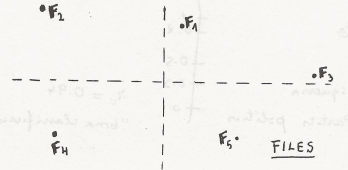
\includegraphics{FILES.png} \(\\\)

\(\\\)

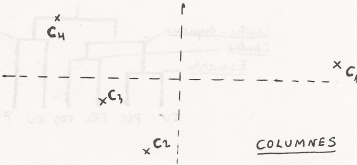
\includegraphics{COLUMNES.png} \(\\\) \(\\\)

\(\\\)El \textbf{vector de medias} de la matriz
\(X = \Bigg(\frac{f_{ij}}{\sqrt{f{.j}} f{i.}} \Bigg)\) es: \[
\overline{X} = (\sqrt {f_{.1}},..., \sqrt{f_{.n}})
\] y la \textbf{matriz de covarianzas} es
\(C_n = X'\cdot D_k \cdot X - \overline{X}'\cdot \overline{X}\) siendo,
como ya hemos dicho, \(D_k = diag(f_{1.},\cdots,f_{k.})\). Es fácil ver
que solo hace falta diagonalizar
\(X'\cdot D_k \cdot X = T \cdot D_{\lambda} \cdot T'\), donde \(T\)
contiene los \textbf{vectores propios} y
\(D_{\lambda} = diag(\lambda_1,\cdots,\lambda_n)\) contiene los
\textbf{valores propios}, los cuales cumplen
\(\lambda_1 = 1 \geq \lambda_2 \geq \cdots \geq \lambda_n \geq 0\). Las
coordenadas de las \emph{filas} son las \emph{columnas} de la matriz \$
A = XT\$, pero la primera columna se omite (debido a que el valor propio
\(\lambda = 1\) de \(X'\cdot D_k \cdot X\) corresponde al valor propio
\(\lambda = 0\) de \(C_n\) y, por tanto, no explica ninguna
variabilidad). \(\\\) \(\\\) Análogamente, consideramos
\(\check{X'} \cdot D_k \cdot \check{X} = \check{T} \cdot D_{\lambda} \cdot \check{T'}\)
i las coordenadas de las \emph{columnas} son las columnas de
\(B = \tilde{X'} \cdot \tilde{T}\), pero solo consideramos a partir de
la segunda. El porcentaje de variabilidad explicado por los ejes \(2\) y
\(3\) es
\(= 100[\frac{(\lambda_2 +\lambda_3)}{(\lambda_2+\cdots+\lambda_n)}]\)

\hypertarget{representaciuxf3n-conjunta}{%
\subsubsection{REPRESENTACIÓN
CONJUNTA}\label{representaciuxf3n-conjunta}}

Las dos representaciones de filas y columnas están relacionadas; se
cumplen las siguientes relaciones entre \(A\) y \(B\): \[
A = {D_k}^{-1} F B {D_\lambda}^{-1/2} \qquad \quad B = {D_n}^{-1} F' A {D_\lambda}^{-1/2}
\]

Las coordenadas (segunda y tercera) de la columna \(C_j\) cumplen : \[
(b_{j2},b_{j3}) = \frac{f_{1j}}{f_{.j}} ({a}_{12}^*,{a}_{13}^*) + \cdots + \frac{f_{kj}}{f_{.j}} ({a}_{k2}^*,{a}_{k3}^*)
\] (siendo \({a}_{ih}^* = {a}_{ih} / \sqrt\lambda_{\nu}\) ) i por tanto
son una \textbf{media} ponderada respecto a las frecuencias relativas
\(f_r (F_i / C_j) = \frac{f_{ij}}{f_{.j}}, \space i = 1,\cdots,k\)) de
las coordenadas (segona y tercera) de las ``filas''.

\begin{longtable}[]{@{}llllllll@{}}
\toprule
FUMADORES & & & & & & &\tabularnewline
\midrule
\endhead
& & No & Flojo & Medio & Fuerte & &\tabularnewline
===================== & ----- & -------- & -------- & -------- &
-------- & ----- & ------\tabularnewline
& & \(C_1\) & \(C_2\) & \(C_3\) & \(C_4\) & &\tabularnewline
Directivos \emph{senior} & \(F_1\) & 4 & 2 & 3 & 2 & 11 &
\(f_1\)\tabularnewline
Directivos \emph{junior} & \(F_2\) & 4 & 3 & 7 & 4 & 18 &
\(f_2\)\tabularnewline
Empleados \emph{senior} & \(F_3\) & 25 & 10 & 12 & 4 & 51 &
\(f_3\)\tabularnewline
Empleados \emph{junior} & \(F_4\) & 18 & 24 & 33 & 13 & 88 &
\(f_4\)\tabularnewline
Secretarios & \(F_5\) & 10 & 6 & 7 & 2 & 25 & \(f_5\)\tabularnewline
& & 61 & 102 & 64 & 25 & N =19 &\tabularnewline
& & \(f_{.1}\) & \(f_{.2}\) & \(f_{.3}\) & \(f_{.4}\) & &\tabularnewline
\bottomrule
\end{longtable}

\begin{figure}
\centering
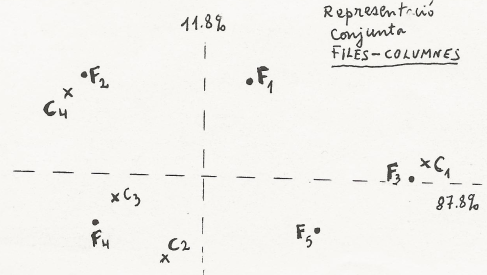
\includegraphics{filcol.png}
\caption{REPRESENTACIÓN CONJUNTA FILAS-COLUMNAS}
\end{figure}

\hypertarget{anuxe1lisis-de-componentes-principales}{%
\subsubsection{ANÁLISIS DE COMPONENTES
PRINCIPALES}\label{anuxe1lisis-de-componentes-principales}}

\hypertarget{definiciuxf3n}{%
\subparagraph{Definición :}\label{definiciuxf3n}}

Dadas \(n\) variables aleatorias observables \(x_1,x_2,\cdots,x_n\), las
componentes principales son \(n\) variables compuestas: \[
Y_1 = t_{11}x_1+\cdots + t_{n1}x_n,\cdots, Y_2 = t_{1n}x_1 + \cdots + t_{nn}x_n
\] tales que (condicionado a la restricción
\(\sum^n_{h=1} {t_{hi}}^2 = 1\)):

\begin{enumerate}
\def\labelenumi{\arabic{enumi})}
\tightlist
\item
  Están incorrelacionadas dos a dos: \(\\\)
  \(corr(Y_i,Y_j) = 0 \qquad i \not= j = 1, \cdots, n\)
\item
  Las variancias son respectivamente máximas: \(\\\)
  \(var(Y_1) = \lambda_1 \geq var(Y_2) = \lambda_2 \geq \cdots \geq var(Y_n) = \lambda_n\)
\end{enumerate}

\textbf{Caso particular n = 2:} \begin{equation}
x_1 ; x_2 \\ 
Y_1 = t_{11}x_1 + t_{21}x_2 \\ 
Y_2 = t_{12}x_1 + t_{22}x_2 \\ 
var(Y_1) = \lambda_1 \geq var(Y_2) = \lambda_2 \\ 
\begin{pmatrix}
t_{11} & t_{12} \\
t_{12} & t_{22} 
\end{pmatrix}
\end{equation} \textbf{verifica}: \[
 T\cdot T' = I_2
\]

\hypertarget{obtenciuxf3}{%
\paragraph{OBTENCIÓ}\label{obtenciuxf3}}

Sea \(S\) la matrix de covarianzas, busaamos los vectores y valores
propios \(S=TDT'\), donde \(T\) es ortogonal y contiene los vectores
propios \(t_1, \cdots, t_n\). Entonces los componentes son: \[
Y_1 = {t_1}^{'}x, Y_2 =  {t_2}^{'}x, \cdots,  Y_n = {t_n}^{'}x 
\] \textbf{NOTA}: primer teorema fundamental tomando \(A=S\) i \(B=I_n\)

\hypertarget{interpretaciuxf3n-geomuxe9trica}{%
\paragraph{INTERPRETACIÓN
GEOMÉTRICA}\label{interpretaciuxf3n-geomuxe9trica}}

Representan las direcciones gozando de máxima variabilidad; \(\\\)

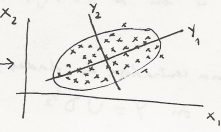
\includegraphics{elipside.png}\(\\\)

\(\\\)donde:

\begin{itemize}
\tightlist
\item
  \(Y_1\) es el primer eje principal de l'elipsoide de concentración
\item
  \(Y_2\) es el segundo eje principal
\end{itemize}

\hypertarget{aplicaciones}{%
\paragraph{APLICACIONeS}\label{aplicaciones}}

\begin{enumerate}
\def\labelenumi{\arabic{enumi}.}
\tightlist
\item
  Reducción de las variables (factores de grandeza, forma, etc\ldots).
  Tomando solo \(m\) componentes \(Y_1, \cdots, Y_n\) la variana
  explicada es \[
  V_m = 100 \times \frac{\lambda_1+ \cdots + \lambda_m}{\lambda_1+ \cdots + \lambda_n}
  \] Las variables iniciales quedan bien representadas por
  \(Y_1, \cdots, Y_m\) si \(V_m\) es grande, por ejemplo, el \(90\%\)
\item
  Reducción de la dimensión en representación de datos:

  \begin{figure}
    \begin{minipage}{.5\linewidth}
   \centering
   \[\left(\begin{array}{cc}
     x_{11} & x_{12} & \cdots & x_{1n} \\
     x_{21} & x_{22} & \cdots & x_{2n} \\
            & \cdots &                 \\   
     x_{N1} & x_{N2} & \cdots & x_{Nn} \\
   \end{array}\right) = X\]
   Matriz de datos original
    \end{minipage}
  $\longrightarrow$
    \begin{minipage}{.5\linewidth}
   \centering
   \[\left(\begin{array}{cc}
     y_{11} & y_{12} & \\
     y_{21} & y_{22} & \\
      \cdots  & \cdots &  \\   
     y_{N1} & y_{N2} & \\
   \end{array}\right) = Y = X \cdot T_2\]
   Matriz de datos transformadas ($m=2$)
    \end{minipage}
    \end{figure}
\end{enumerate}

\end{document}
